\documentclass[11pt]{article}
\usepackage{fullpage}
\usepackage[utf8]{inputenc}
% \usepackage{algorithm}
% \usepackage{algorithmic}
\usepackage{amsfonts}
\usepackage{graphicx}
\usepackage{amsthm}
\usepackage{mathrsfs}
\usepackage{amssymb}
\usepackage{hyperref}
\usepackage{amsmath}
\usepackage{cite}
\usepackage{xcolor}
\newtheorem{theorem}{Theorem}
\newtheorem{lemma}{Lemma}
\newtheorem{definition}{Definition}
\newtheorem{claim}{Claim}
\newtheorem{corollary}{Corollary}
\newtheorem{observation}{Observation}
\newtheorem{remark}{Remark}
\newtheorem{oq}{Open Question}
\usepackage[normalem]{ulem}

% \usepackage{algorithm}
\usepackage{algpseudocode}
% \usepackage{aligned-overset}
% \usepackage{fontspec}
% \algrenewcommand\algorithmicrequire{\textbf{Precondition:}}
% \algrenewcommand\algorithmicensure{\textbf{Postcondition:}}
% \usepackage{xfrac}
% \usepackage{setspace}


\usepackage{algorithm}
\usepackage{algpseudocode}


% images
\usepackage{graphicx}
\graphicspath{ {./images/} }


\begin{document}
\title{Final Project - Distributed Graph Algorithms - Spring 2022\\
On the paper: "Can We Break Symmetry with $o(m)$ Communication?", by Shreyas Pai, Gopal Pandurangan, Sriram V. Pemmaraju, Peter Robinson
}
\author{Rotem Shavitt\footnote{rotemshavitt@campus.technion.ac.il, 209638162} \and Ido Frankel\footnote{ido.frankel@campus.technion.ac.il, 318985108}
}
\date{\today}
\maketitle

\section{Summary}

The article discusses the message complexity in distributed symmetry breaking problems, aiming specifically at $\Delta + 1 $ coloring and MIS problems. In global problems, it has been proven that $\Omega(m)$ messages are a lower bound with no additional assumptions. Knowing this, the authors are trying to answer whether this bound implies to local problems as well, or whether sublinear message complexity (i.e. $o(m)$) is possible for problems such as $\Delta +1$ coloring and MIS. The results are achieved in three different congest models, KT-1, KT-2 and the general model KT-$\rho$, (which stands for starting knowledge of neighbor's IDs till radius $\rho$).

\subsection*{Lower Bound}

The paper suggests 2 constructions of designated graphs in order to prove $\Omega(m)$ and $\Omega(n)$ lower bounds in KT-1 and KT-$\rho$ (for $\rho \ge 2$), respectively. 
\begin{figure}[h]
    \centering
    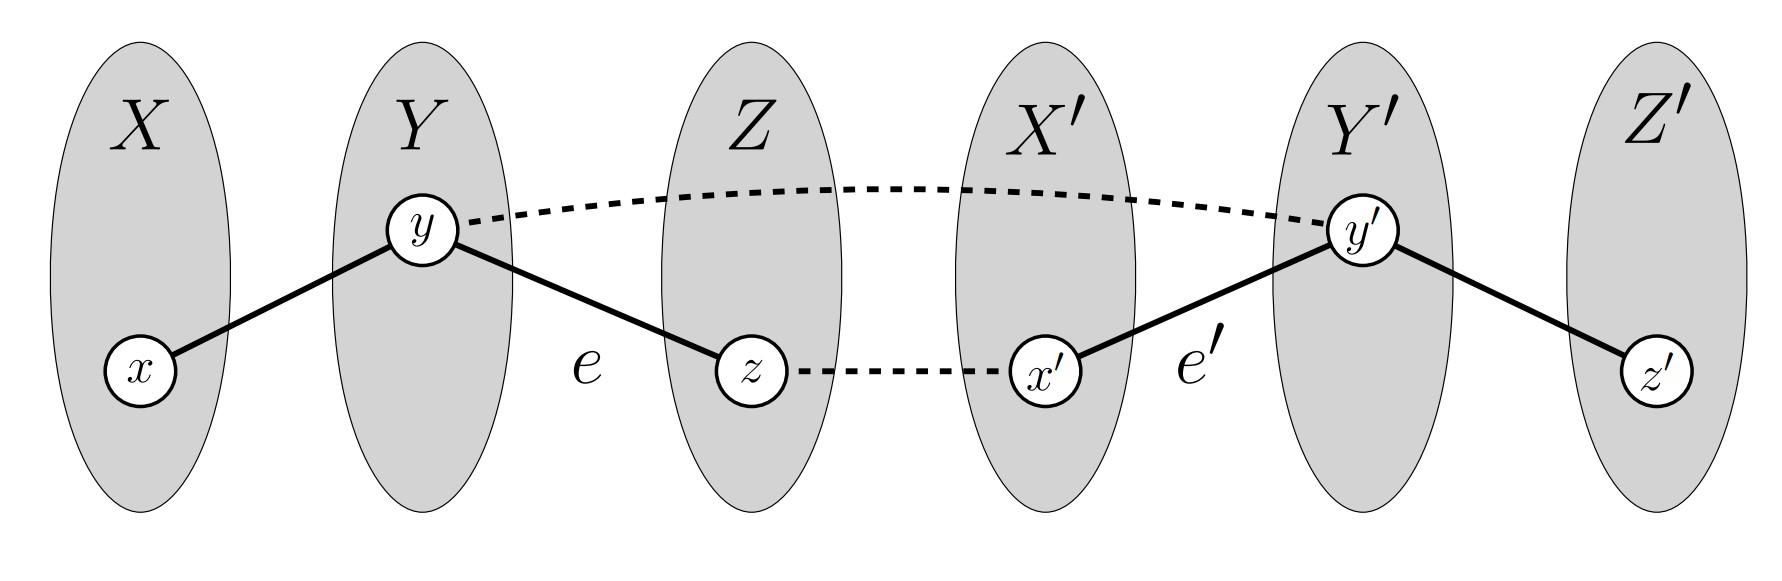
\includegraphics[scale=0.7]{graph_cross_graph}
    \caption{base graph $G \cup G'$, and the crossed graph $G_{e,e'}$ (dashed) taken from the article}
    \label{fig:graph_cross_graph}
\end{figure}
First, the paper suggests a \textit{Base Graph} $G \cup G'$, where $G$ = $( X \cup Y \cup Z, E)$, in which $X \cup Y$, $Y \cup Z$ are complete bipartite graphs, and $G'$ is a copy of $G$. 
Then, we create a \textit{crossed graph} $G_{e,e}'$, as follows: 
We remove $e=(y,z)$ and $e'=(x',y')$ from the \textit{base graph}, and add $(z,x'), (y,y')$ which closes a cycle with $e,e'$. The authors then show that the previous graphs are similar in terms of executions for any comparison-base algorithm. They relies directly on the lemmas and definitions introduced by Awerbuch et al.\cite{Awerbuch}, which we will briefly introduce, In their paper they define an edge $(u,v)$ as utilized during an execution if a message is sent on it or if either $u, v$ sends or receives a message containing the other edge-end vertex ID assignment.

Awerbuch et al. showed that if pair of crossing edges $e, e'$ are not utilized during the execution by a comparison algorithm, then the executions of the touching nodes in both graphs are similar.

The article relies on the execution's similarities in order to show that by well-chosen edges in the graph, a contradiction can be achieved with respect to the correctness of problems such as $\Delta +1$ coloring and MIS. The contradiction then imposes a constraint on the comparison algorithm itself, which leads to the desired lower bounds.

In order to show the $\Omega(m)$ for the $(\Delta +1)$-coloring in KT$-1$ congest model, the authors suggest two different ID assignments $\phi, \psi$, for the base graph and the crossed graph, respectively. They then use the fact that $G$ and $G'$ are isomorphic in order to show that the execution $EX_G$ and $EX_{G'}$ are similar for every $v$ and $v'$. Later, based on the definition of $\psi$ the authors show that every vertex in $G$ and its counterpart in $G'$ have the same local state under $\psi$. Because $EX$ and $EX_{e,e'}$ are similar, it means that they have the same color. The contradiction is achieved by picking specific vertices $y,y'$ which are neighbors in the crossed graph, hence must not have the same color.

Next, the article proves a lower bound of $\Omega(n)$ in expectation w.h.p. in the KT-$\rho$ model for any randomized Monte Carlo algorithm.
The proof presented in the article relies on previous work by by Linial \cite{Linial}, and Naor \cite{Naor} which present a lower bound on the rounds for any probabilistic algorithm for 3-coloring and MIS. The paper uses their results to present a lower bound of $\Omega(n)$ messages. It presents a graph $G$ consisting of a disjoint union of $\frac{n}{k}$ cycles (each of $k$ nodes, where $k$ is a constant defined in the paper). The authors assume by contradiction there exists an algorithm which sends sublinear amount of messages, since there are $\Omega(n)$ cycles, it holds that with high probability there exists a cycle which all of its nodes, do not send any message. Meaning, the output of such node is based on its initial knowledge which consists of the random choice of color, and its neighborhood. Because the behavior follows the same probability distribution under both KT-$\rho$ and KT-$0$, it implies that with high probability there exist two nodes in the cycle that produce the same color.

\subsection*{Upper Bound}
The article presents 3 new algorithms that improve message complexity under different circumstances. Two of them are for coloring problems and another for finding MIS.

\subsubsection*{Coloring}

The first algorithm presented uses the assumption of the KT-1 model and creates a $(\Delta+1)$ coloring solution in ${\Tilde{O}}(D+\sqrt{n})$ rounds with complexity of ${\Tilde{O}}(n^{1.5})$ messages. It is partitioning all vertices into $L, B_1, B_2, ..., B_k$ disjoint sets, and all color are divided into $C_1, C_2, ..., C_k$ uniformly. The Idea behind it is to run Johannson's \cite{Johansson} randomized coloring algorithm on a small enough partition in order to use only the corresponding color pallet. 

At first They Build a sparsified spanning subgraph $H$. Then, in each $B_i$ the nodes will execute a randomized algorithm for coloring by Johansson \cite{Johansson}. Then, until $G[L]$ has $\Tilde{O}(n)$ edges (which can be checked by using $H$), they recursively run the algorithm on $G[L]$ and finish.

The next algorithm shows how in the KT-1 CONGEST model when we drop the demand for $(\Delta+1)$ coloring solution and instead solve a $(1+\epsilon)\Delta$ coloring solution, we can improve message complexity to $\Tilde{O}(n/\epsilon^2)$. This algorithm works for any $\epsilon$ but is an improvement for higher values of $\epsilon$.
In each phase of the algorithm, every node chooses randomly a potential color, check if that choice is valid with respect to it's neighbors coloring, and if so determines it to be it's final color and deactivates. W.h.p, all the nodes are assigned a color after $O(\frac{\log{n}}{\epsilon})$ rounds. In each round, the active nodes needs to communicate with their active neighbors, counting to be $O((\log{n})^{2}/ \epsilon)$ w.h.p, summing into the message complexity $\Tilde{O}(n/\epsilon^2)$.

\subsubsection*{MIS}

The last algorithm presented in the article is an MIS algorithm that works in the KT-2 congest model. First, a set of $O(\sqrt{n})$ vertices is chosen as the starting input of a randomized greedy MIS algorithm. Each vertex $v$ that enters the MIS now needs to inform all $v$'s neighbors in order for them to deactivate themselves. In addition, we want to inform $v$'s 2-hop neighbors that their neighbors were deactivated. For this we use the additional knowledge of the KT-2 model. Because all the vertices of max distance 2 from $v$ know each other's IDs, they can calculate a BFS tree in $O(1)$. We use this tree to transfer messages instead of broadcasting which may cause a redundancy of messages sent. After the graph has been updated accordingly, they run Luby's \cite{Luby} algorithm on the remnant graph. In total, the message complexity achieved by this algorithm is $\Tilde{O}(n^{1.5})$.

\subsubsection*{conclusion}
The article managed to prove that without additional assumptions to the knowledge of the KT-1 model, sublinear message complexity is not possible for $(\Delta + 1)$ coloring and MIS problems while using comparison-based algorithms. However, for non-comparison-based algorithm it presents a new coloring algorithm, which achieves sublinear message complexity. If we ease the problem into $(1+\epsilon)\Delta$ coloring, the article presents another non-comparison-based algorithm that achieves an even better message complexity (for certain $\epsilon$ values). For the MIS problem, by simply using the KT-2 model (instead of KT-1) the authors managed to compose an algorithm that reaches the desired sublinear message complexity.
\newline


\section{Related Work}
Most of the papers which discuss local problems that precede this article are revolved around round complexity bounds. Therefore, the results of the article are not an improvement of previous work, but a new angle for solving local problems.

On the other hand, there exist papers which discuss message complexity in global problems. One fundamental paper is of Awerbuch et al.\cite{Awerbuch} which discussed time-message trade-offs in many fundemental distributed graph problems. In the paper it's shown that $\Omega(m)$ is a lower bound for broadcasting and spanning trees problems for comparison-based algorithms. In their paper Awerbuch et al. defined the terms of \textit{execution} of a protocol, and \textit{similarities} in order to show an equivalence between two algorithms. In addition the paper suggests a construction of a special family of network graphs (i.e. \textit{crossed graph}) for their lower bounds proof. Our paper pushed farther the construction of Awerbuch et al. and uses definitions which were initially defined in their paper in order to prove lower bounds in local problems.
Many years later, King et al. \cite{King} showed that by lifting the restriction of comparison-based algorithm and using a polynormal size ID space, the lower bounds presented by Awerbuch et al. breaks. In their article they focus on Spanning trees and minimum spanning trees. As proven in Theorem 1.1 in \cite{King}, there are algorithms who succeede w.h.p. in a synchronous networks to construct a minimum spanning tree (MST) using time and messages $O(\frac{n\log^2{n}}{\log{\log{n}}})$ and to construct spanning tree (ST) with $O(n\log{n})$ messages. Those algorithm works in the KT-1 Congest model.

The work described above left question on local symetry

\section{New Results}
Our efforts have been concentrated on applying ideas presented in the article on other local problems and problems with different initial assumptions. We'll present 2 new algorithms, the first is a variation of the paper's second algorithm for $(\epsilon+1)\Delta$-coloring. Since it was proven in the paper that it's impossible to obtain an $o(m)$ message complexity using non-comparison based algorithm in the KT-1 model, we wanted to see which other easing assumption can help us obtain sublinear message complexity in coloring problem. We came up with a $p$-defective $(\Delta+1)$-coloring algorithm in the KT-1 model which exchanges $O(n \frac{\log^3{n}}{\log^2{\frac{p-1}{2}}})$ messages w.h.p.
In addition we explored the ruling set problem, which is a generalization of the MIS problem, and constructed a $(k, k\log{n})$-ruling Set algorithm in the KT-$2(k-1)$ model, obtaining $O(n\cdot\Delta^k\log{n})$ message complexity. 

\subsection{\texorpdfstring{p-defective $(\Delta+1)$-coloring using $O(n \frac{\log^3{n}}{\log^2{\frac{p-1}{2}}})$ messages in KT-1 Congest model}{}}

\subsubsection*{Setting}
% Similarly to what was shown in the article, at the beginning of the algorithm one node generates a string of  $C \cdot \log^2{n} \cdot \frac{\log{n}}{\log{\frac{p-1}{2}}}$ random bits and shares it with all the other nodes using a danner, which is a sparsified spanning subgraph of the original graph \cite{Gmyr}. This takes $\Tilde{O}(\frac{n}{\log{\frac{p-1}{2}}})$ messages and $\tilde{O}(n)$ rounds in the KT-1 Congest model, as shown in corollary 1.2 in the paper (\textbf{TODO, VERIFY ROUNDS AND MESSAGE COMPLEXITY, NOT SURE}). Each node $v$ that has not already permanently colored itself, will use random bit string $s_i$ of length $\Theta(\log^2{n}$) in phase $i$ in order select a random hash function $h_i$ from a family of $\Theta(\log{n})$-wise independent hash functions $\mathcal{H}=\{h:[\text{poly}(n) \xrightarrow{} [\Delta+1] \}$. The color chosen by each node would be the result from applying $h_i$ on the ID, which makes the KT-1 knowledge crucial for knowing the potential colors rolled by the neighbors.

Similarly to what was shown in the article, at the beginning of the algorithm one node generates a string of  $C \cdot \log^2{n} \cdot \frac{\log{n}}{\log{\frac{p-1}{2}}}$ random bits and shares it with all the other nodes using a danner, which is a sparsified spanning subgraph of the original graph \cite{Gmyr}. This takes $\Tilde{O}(n^{1+\epsilon}\cdot \epsilon)$ messages and $\tilde{O}(\frac{n}{\epsilon})$ rounds (for $ 1 > \epsilon > \log{\log{n} / \log{n}} $) in the KT-1 Congest model, as shown in corollary 1.2 in the paper and explained in article \cite{Gmyr}. Each node $v$ that has not already permanently colored itself, will use random bit string $s_i$ of length $\Theta(\log^2{n}$) in phase $i$ in order select a random hash function $h_i$ from a family of $\Theta(\log{n})$-wise independent hash functions $\mathcal{H}=\{h:[\text{poly}(n) \xrightarrow{} [\Delta+1] \}$. The color chosen by each node would be the result from applying $h_i$ on the ID, which makes the KT-1 knowledge crucial for knowing the potential colors rolled by the neighbors.



\begin{algorithm}
\caption{p-defective $\Delta+1$-coloring (One round)}
\begin{algorithmic}[1]
\State Each active vertex chooses a random $S_i$ string, computes the candidate color to be $h_i(v.id)$ and send to all neighbors.
\If{v isn't colored}
    \State \textbf{if} not more than $p$ of $v$'s neighbors have picked the same color \textbf{and} no neighbor disapproved, $v$ colors itself and notify the neighbors.
\Else
    \State \textbf{if} $v$ have more than $p$ neighbors with his color, send disapproval to neighbors.
\EndIf
\end{algorithmic}
\end{algorithm}

\begin{lemma}
\label{prob_pick_good_color}
Each vertex chooses a color, which was picked by at most $p-1$ of its neighbors with probability of $\frac{d}{(1+\Delta) \cdot p}$
\end{lemma}
For any of $v$'s neighbors (denote $d$ as the amount of $v$'s neighbors), let $X_{u_i}$ be an indicator variable that indicates if a neighbor $u_i$ has picked the same color as $v$. Then $P(X_{u_i}) = \frac{1}{1 + \Delta}$. Let $X_v = \sum{X_{u_i}}$. By Markov's inequality $P(X_v \ge p) \le \frac{E(X_v)}{p} = \frac{d}{(1+\Delta) \cdot p}$.

\begin{lemma}
\label{rounds}
A vertex successfully colors itself in $O(\frac{\log{n}}{\log{\frac{p-1}{2}}})$ rounds w.h.p.
\end{lemma}

\begin{gather*}
P(v \text{ hasn't been color in round } i)\\ 
= P([v \text{ has at least p neighbors with same color as his }] \bigcup \; [\exists u\in N(v): c(v)=c(u) \land u \text{ rejects}]) \\
\underset{\text{Inclusion–exclusion}}{=} P(\underset{A}{\underbrace{x_v \ge p}}) + P(\underset{B}{\underbrace{\exists u\in N(v): c(v)=c(u) \land u \text{ rejects}}}) - P(A \bigcap B) \le P(A) + P(B) \\
= P(\underset{A}{\underbrace{x_v \ge p}}) + P(\overset{B}{\overbrace{\bigcup_{u \in N(v)} c(v)=c(u) \land u \text{ rejects}}}) \\
\underset{\text{U.B}}{\underbrace{\le}} P(x_v \ge p) + \sum_{u \in N(v)}{P(c(v)=c(u) \land x_u \ge p)} \\
=  P(x_v \ge p) + \sum_{u \in N(v)}{P(c(v)=c(u)) \cdot P(X_u \ge p \mid c(u) = c(v))} \\
= P(x_v \ge p) + \sum_{u \in N(v)}{\frac{1}{1 + \Delta} \cdot \frac{d_{u}-1}{(1+ \Delta) \cdot (p-1)} }
\end{gather*}

\begin{gather*}
\le \frac{\Delta}{(\Delta + 1) \cdot p} + \sum_{u \in N(v)}{\frac{1}{1 + \Delta} \cdot \frac{\Delta-1}{(1+ \Delta) \cdot (p-1)} } \\
\le \frac{\Delta}{(\Delta + 1) \cdot p} + \frac{\Delta^2}{(1 + \Delta)^2 \cdot (p-1)}
\le \frac{1}{p} + \frac{1}{p-1} \le \frac{2p}{p(p-1)} = \frac{1}{\frac{p-1}{2}}
\end{gather*}
Thus, the probability that $v$ does not color itself in $O(\frac{\log{n}}{\log{\frac{p-1}{2}}})$ rounds is:

\begin{gather*}
P(v \text{ wasn't colored in $O(\frac{\log{n}}{\log{\frac{p-1}{2}}})$ rounds})
\le [(\frac{p-1}{2})^{-1}]^{c \cdot \frac{\log{n}}{\log{\frac{p-1}{2}}}}
= [(\frac{p-1}{2})^{-1}]^{\log_{\frac{p-1}{2}}{n^c}}= n^{-c} \\
P(\exists v \text{ which hasn't been colored}) = P(\bigcup_{i} v_i \text{ has not been colored}) \\
\underset{U.B}{\underbrace{\le}} \sum_{i}^{n} P(v_i \text{ hasn't been colored}) = n \cdot n^{-c} = n^{1-c} \\
\end{gather*}

Thus, the probability that all vertices have been colored is
\begin{gather*}
P(\textbf{all vertices have been colored}) = 1 - n^{1-c} = 1 - \frac{1}{n^{c-1}} = 1 - \frac{1}{n^{c'}}
\end{gather*}
Hence w.h.p. all vertices have been colored in  $O(\frac{\log{n}}{\log{\frac{p-1}{2}}})$ rounds. 

\begin{lemma}
\label{A_2_APPENDIX}
Suppose that $X$ is the summation of $n$, $c$-wise independent 0-1 random variables, each with mean $p$, let $\mu$ satisfy $\mu \ge \mathbb{E}[X] = np$. Then $Pr[X \ge (1+\delta)\mu] \le exp(-\min{c, \delta^2 \mu})$
\end{lemma}
Taken from lemma A.2 from the paper's appendix.

\begin{lemma}
\label{colors_conflict}
There are at most $\log{n}$ vertices which could have picked same color $c$ as $v$ in every round.
\end{lemma}
In step 2, a vertex will check if not more than $p$ of its neighbors have picked same color as itself, it will only check neighbors that could have chosen this color in this round or in any previous rounds. Because each vertex chooses hash function $h_i$ according to the corresponding $s_i$, which is shared by all vertices, as described in the setting. Under $KT-1$ congest model, each vertex knows its neighbors' ID, hence it can locally calculates which of its neighbors could have picked the same color as itself.

By Lemma \ref{prob_pick_good_color}, $E(x) = \frac{d}{1 + \Delta}$. Since the colors of the vertices are chosen using an $\Theta(\log{n})$-wise independent family of hash functions $\mathcal{H}$, then the indicators $X_{u_i}$, themselves (which represents whether a neighbor has picked same color $c$ as $v$) are $\Theta(\log{n})$-wise independent. By lemma \ref{A_2_APPENDIX} , it holds w.h.p. there are at most $O(\log{n})$ neighbors of $v$ which could have picked the same color $c$ as $v$ in this round. 

\begin{lemma}
\label{message_per_round}
In each round, each vertex exchanges $O(\frac{\log^2{n}}{\log{\frac{p-1}{2}}})$ messages.
\end{lemma}
By lemma \ref{colors_conflict}, in each round $v$ can have a conflict with $O(\log{n})$ of its neighbors. $v$ has to check his coloring with all of the neighbors who could have picked this color in this round and in all previous rounds. By lemma \ref{rounds} there are $O(\frac{\log{n}}{\log{\frac{p-1}{2}}})$ rounds w.h.p. Therefore $v$ has to check with not more than $O(\frac{\log^2{n}}{\log{\frac{p-1}{2}}})$ vertices w.h.p. in each round.

% Hence $v$ has to check all of its $O(\log{n})$ neighbors which have chosen color $c$ in this round or prior rounds \textbf{WHY, ALSO PRIOR ROUND MAKE SURE THE CORRECTION OF THE ALGORITHM STILL HOLDS, IF TAKING INTO ACCOUNT PREVIOUS ROUNDS} to be sure that there isn't a situation where more than $p$ of its neighbors have picked same color as $c$ in same round. Since there are $O(\frac{\log{n}}{\log{\frac{p-1}{2}}})$ rounds w.h.p (according to lemma \ref{rounds}), color $c$ is chosen by only $O(\frac{\log^2{n}}{\log{\frac{p-1}{2}}})$ neighbors w.h.p during the algorithm.

\begin{theorem}
The algorithm exchanges $O(n\cdot \frac{\log^3{n}}{\log^2{\frac{p-1}{2}}})$ messages
\end{theorem}
By lemma \ref{message_per_round}, each vertex exchanges $O(\frac{\log^2{n}}{\log{\frac{p-1}{2}}})$ messages per round, By lemma \ref{rounds}, there are $O(\frac{\log{n}}{\log{\frac{p-1}{2}}})$ rounds w.h.p. Hence the total message complexity (for all vertices) is $O(n\cdot \frac{\log^3{n}}{\log^2{\frac{p-1}{2}}})$
\newline
\newline

\subsection{\texorpdfstring{$(k, k\log{n})$-Ruling Set using $O(n\cdot\Delta^k\log{n})$ messages in KT-$2(k-1)$ Congest model}{}}

% \subsubsection*{Setting}
This algorithm finds a $(k, k\log{n})$-Ruling Set for any $U\subseteq V$. This algorithm runs in iterations on the indices of the IDs, meaning all the ID's needs to be shifted to the range of $[1,n]$. In each iteration of the algorithm, the vertices who withholds a certain criteria notify all vertices within distance $2(k-1)$ because they might need to remove themselves. In order to minimize the message complexity, instead of simply broadcasting the ID for $k$ rounds, the vertices would compute a $BFS$ tree and would send messages only on it's edges, meaning every node would receive only one message from each root. In algorithm 3 in the article, the nodes use the $KT-2$ knowledge in order to compute internally the depth 2 $BFS$ tree and inform efficiently all 2-hop neighbors. We were inspired by that idea and extended it to a $k$-depth tree, which would use the KT-$2(k-1)$ knowledge.

\begin{algorithm}
\caption{$(k, k\log{n})$-Ruling Set:}
\begin{algorithmic}[1]
\State $\forall u\in U: u\in R$.
\For {$i\in [1,log{n}]$}
    \If{$v.id[i] = 1$ and $v\in R$}
        \State send self $id$ to the computed $BFS$ tree of depth $2(k-1)$
    \EndIf
    \If{$u$ received $v.id$}
        \State send $v$'s ID in $v$'s $BFS$ tree
        \If{$v.id[i] = 0 $}
            \State remove self from $R$
        \EndIf
    \EndIf
\EndFor
\end{algorithmic}
\end{algorithm}


\begin{lemma}
\label{bfs_tree}
All vertices in $u$'s $BFS$ tree within distance $k$ receive the ID message after $k$ rounds of forwarding with $O(\Delta^k)$ messages in total. 
\end{lemma}
We'll first explain and prove how in KT-$(2k-2)$ model a depth k $BFS$ tree can be computed with no additional messages.
Every node which receive an ID message can infer it's distance $d$ from the root by the number of rounds passed from the beginning of the round. Every node at distance $d+1$, holds that it's father in the $BFS$ tree would be the node of distance $d$ with the lowest ID.


A node $v$ of distance $d<k$ knows all other potential fathers of a neighbor $u$: 
All potential fathers for $u$ are it's neighbor, therefore of distance from $v$ and within knowledge range. In addition, all other nodes of distance $d$ from the root are from max distance $2\cdot d$ from $v$, hence that is the distance of the route through the root, and because $2\cdot d\le 2(k-1)$, withing knowledge distance, meaning the father of each node in the tree can be determined solely on the KT-$(2k-2)$ knowledge.


Having the computed tree, every node forwards the ID received to It's children in the tree, meaning the all the nodes are informed after $k$ rounds. Each node receives a message only from it's father, therefore the amount of messages sent is the size of the tree, meaning $O(\Delta^k)$ messages.

\begin{lemma}
\label{alpha_rule}
$\forall u,v \in R, d(u,v) \ge k$.
\end{lemma}
Assume by contradiction that $\exists u,v\in R: d(u,v)<k$.
$u,v$ have distinct IDs, therefore they must differ in at least one bit. Let i be the first bit that differs. w.l.o.g $u.id[i]=1, v.id[i]=0$. Then in the $i_{th}$ iteration, $u$ withholds the condition, therefore would send self ID to the $BFS$ of depth $2(k-1)$ rooted in $u$. By lemma \ref{bfs_tree} if $d(u,v)<k$, then $v$ would receive $u$'s ID, and by algorithm would remove itself from $R$, which is a contradiction to the initial assumption.

\begin{lemma}
\label{beta_rule}
$\forall u\in U,\exists r\in R, \text{ s.t } d(u,r) \le k$
\end{lemma}
We'll prove by induction that in the beginning of the $i_{th}$ iteration, $\forall u \in U,\: \exists r\in R, \text{ s.t } d(u,r) \le (i-1)k$.

\textbf{Base}: $i=1$, by the definition of the algorithm, before the first iteration $\forall u\in U: u\in R$, therefore $d(u,u)=0\le 1 \cdot k$.


\textbf{Step}: we’ll assume correctness for $i$ and show for $i+1$:
let $u\in U$, by induction assumption $\exists r\in R$ s.t. $d(u,r)\le (i-1)\cdot k$. Divide into cases for the end of the $i_{th}$ iteration
\begin{itemize}
    \item $r\in R$: hence the assumption holds.
    \item $r \notin R$: hence $r$ was removed from $R$. Meaning, in the beginning of the $i_{th}$ iteration, $\exists r'\in R$ s.t. $r'$ initiated a message with $r'$ ID, which $r$ received. According to the algorithm $r'.id[i]=1 \land r'\in R$. By lemma \ref{bfs_tree} since a message was received, at the end of the $i_{th}$ iteration it holds $d(r',r)\le k$. Thus, $d(r',u)\le d(r',r)+d(r,u)\le k+(i-1)\cdot k=i\cdot k$. In addition at the end of the iteration, $r' \in R$, as it holds $r'.id[i]=1$. Hence the induction assumption holds.
\end{itemize}
In the beginning of a hypothetical $\log{n}+1$ iteration, (i.e at the end of the $\log{n}$ iteration), $\forall u\in U, \: \exists r\in R, \text{ s.t } d(u,r) \le (\log{n}+1-1)\cdot k = k\cdot\log{n}$.

\begin{theorem}
\label{final_claim}
The algorithm computes a correct $(k, k\log{n})$-ruling set in $O(\log{n})$ rounds using $O(|U|\cdot\Delta^k\log{n})$ messages.
\end{theorem}
by lemma \ref{alpha_rule} and lemma \ref{beta_rule} we conclude that by definition the result is a correct $(k, k\log{n})$-ruling set. The algorithm runs in iterations on the nodes ID strings, therefore runs in $\lceil{\log{n}}\rceil$ rounds. In each round, there can be $|U|$ different $BFS$ trees since only nodes in $R$ can be the root of one. By lemma \ref{bfs_tree} the amount of messages sent is at most $|U|\cdot \Delta^k$, and the total message complexity of the algorithm is $O(|U|\cdot\Delta^k\log{n})$.

\subsection{conclusion}
We showed in this section two algorithms for breaking symmetry problems with sub-linear message complexity as desired.

In the first algorithm we showed how we can change the assumption while remaining sub-linear message complexity under certain assumptions. Instead of extending the color pallet to $(1 + \epsilon) \cdot \Delta$ as done in the article, we reduced it back to a pallet of size $(1+ \Delta)$ and chose to ease other aspect of coloring, by creating defective coloring as introduced in the course tutorials.

The second algorithm is a generalization of the MIS problem. For $U=V$ and when the graph holds that $\Delta^k < \frac{n}{\log{n}}$, the message complexity is:
\begin{gather*}
O(|U|\cdot \Delta^k\log{n}) = O(n\cdot\Delta^k\log{n}) < O(n\cdot \frac{n}{\log{n}}\cdot \log{n}) \\
\Rightarrow \boxed{O(|U|\cdot \Delta^k\log{n}) = o(m)}
\end{gather*}


\newpage

\bibliographystyle{alpha}
\bibliography{bib-filename}

\begin{thebibliography}{9}
\bibitem{Awerbuch}
Baruch Awerbuch, Oded Goldreich, David Peleg, and Ronen Vainish. 1988. A Tradeoff between Information and Communication in Broadcast
Protocols. 319 LNCS, 2 (1988), 369–379. https://doi.org/10.1007/BFb0040404

\bibitem{Linial}
Nathan Linial. 1992. Locality in Distributed Graph Algorithms. SIAM J. Comput. 21, 1 (1992), 193–201. https://doi.org/10.1137/02210

\bibitem{Naor}
Moni Naor. 1991. A Lower Bound on Probabilistic Algorithms for Distributive Ring Coloring. SIAM J. Discret. Math. 4, 3 (1991), 409–412. https://doi.org/10.1137/0404036

\bibitem{Johansson}
Ojvind Johansson. 1999. Simple Distributed ($\Delta$ + 1)-Coloring of Graphs. Information Processing Letters 70 70 (1999), 229–232.

\bibitem{Luby} Michael Luby. 1985. A Simple Parallel Algorithm for the Maximal Independent Set Problem. In Proceedings of the Seventeenth Annual ACM Symposium on Theory of Computing (STOC ’85). 1–10. https://doi.org/10.1145/22145.22146

\bibitem{King} Valerie King, Shay Kutten, and Mikkel Thorup. 2015. \href{https://doi.org/10.1145/2767386.2767405}{Construction and Impromptu Repair of an MST in a Distributed Network with o(m) Communication}

\bibitem{Gmyr}
Robert Gmyr and Gopal Pandurangan. 2018. \href{https://doi.org/10.4230/LIPIcs.DISC.2018.32}{Time-Message Trade-Offs in Distributed Algorithms}. In 32nd International Symposium on Distributed Computing, DISC 2018, New Orleans, LA, USA, October 15-19, 2018 (LIPIcs), Ulrich Schmid and Josef Widder (Eds.), Vol. 121. Schloss Dagstuhl-Leibniz-Zentrum für Informatik, 32:1–32:18. 
\end{thebibliography}
    

\end{document} 
